\begin{frame}{Синтез системы автоматического управления}
    \begin{itemize}
        \item <+-> []
        \item <+-> []  \begin{block}{Задачи раздела}
                Расчет коэффициентов и моделирование системы стабилизации вертикальной скорости самолета для Concorde: 
            \begin{itemize}
                \item Выбор параметров привода 
                \item Расчет и оценка коэффициентов обратных связей и коэффициентов стабилизации системы
                \item Частотный анализ контуров системы 
                \item Моделирование и анализ линейной и нелинейной САУ
            \end{itemize}
        \end{block}
    \end{itemize}
\end{frame}

\begin{frame}{Исследуемая модель} %Какаета ошибка
    $$ \begin{cases}
            \dot{\alpha}=\omega_z-\bar{Y}^{\alpha} \alpha \\
            \dot{\omega}_z=\bar{M}_z^{\alpha} \alpha+\bar{M}_z^{\omega_z} \omega_z +\bar{M}_z^{\dot{\alpha}} \dot{\alpha}+\bar{M}_z^{\delta_{\text{в}}} \delta_{\text{в}} \\
            \dot{V_y}=V \cdot \bar{Y}^{\alpha} \alpha
    \end{cases} $$ \\
    $A = \begin{pmatrix}
        -\bat{Y^{\alpha}} & 1 & 0\\ 
        \bar{M}_z^\alpha & \bar{M}_z^{\omega_z} & 0\\ 
         V \cdot \bar{Y}^\alpha& 0 & 0 
    \end{pmatrix}$;
    $B = \begin{pmatrix}
     0 \\ 
     \bar{M}_z^{\delta_{\text{э}}} \\ 
     0 
    \end{pmatrix}$ ;
    $C= \begin{pmatrix}
    1 & 0 & 0\\ 
    0 & 1 & 0\\ 
     0& 0 &1 
    \end{pmatrix}$;
    $D = \begin{pmatrix}
     0 \\ 
     0 \\ 
     0 
    \end{pmatrix}$
\end{frame}

\begin{frame}{Структурная схема системы стабилизации вертикальной скорости самолета}
    \center{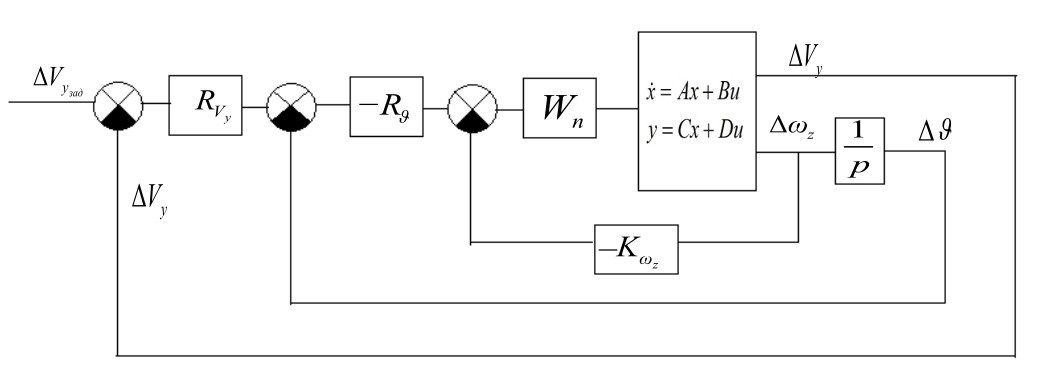
\includegraphics[width = \linewidth]{../Оглавление/Part2/Sactions/Content/figures/Схема.jpg}}
\end{frame}

\begin{frame}{Выбор параметров привода}
    \begin{itemize}
    \item <+-> []
    \item <+-> []   \begin{block}{Передаточная функция привода}
        При решении задачи синтеза сервопривод описывается передаточной функций колебательного звена:
    
    \begin{equation}
    \label{eq:Привод ограничеия}
        W_{\text{п}}=\frac{1}{T_\text{п}^2p^2+2\xi_\text{п}T_\text{п}p+1}
    \end{equation}
    
    Значение постоянной времени  $T_\text{п}$ сервопривода, от которой зависит его полоса пропускания, определяется следующим образом:
    
    Устанавливается максимальное значение собственной частоты  недемпфированных колебаний $\omega_0=\frac{1}{T_{\text{с}}}$ в варианте управлении продольным движением самолета, и исходя из этих значений, определяется потребная ширина полосы пропускания сервопривода (см. формула \ref{eq:Привод ограничеия}):
    \end{block}
\end{itemize}
\end{frame}

\begin{frame}{Выбор параметров привода}
    \begin{block}{Вывод}
        \begin{itemize}
            \item Максимальное значение $\omega_0$ находится у поверхности земли со значением $M = 1$ ($\omega_0_{max} = 5,74 \ \frac{1}{c}$).
            \item $\omega_\text{п} = 37,19 \ \frac{1}{c}$ => $T_{\text{п}} = 0.0269 \ c$ 
            \item Из данного ряда чисел [0,02; 0,025; 0,003; 0,035; 0,04; 0,045; 0,05] 0,0269 более близко к 0,025, следовательно, данное число мы и примем за постоянную времени привода. Исходя из вышесказанного, получаем $\omega_\text{п} = 40 \ \frac{1}{c}$ , $T_{\text{п}} = 0.025 \ c, \xi = 0,5$.
        \end{itemize}
    \end{block}
\end{frame}


\begin{frame}{Расчёт коэффициентов стабилизации системы}
    \begin{minipage}[c]{0.45\textwidth}
        \center{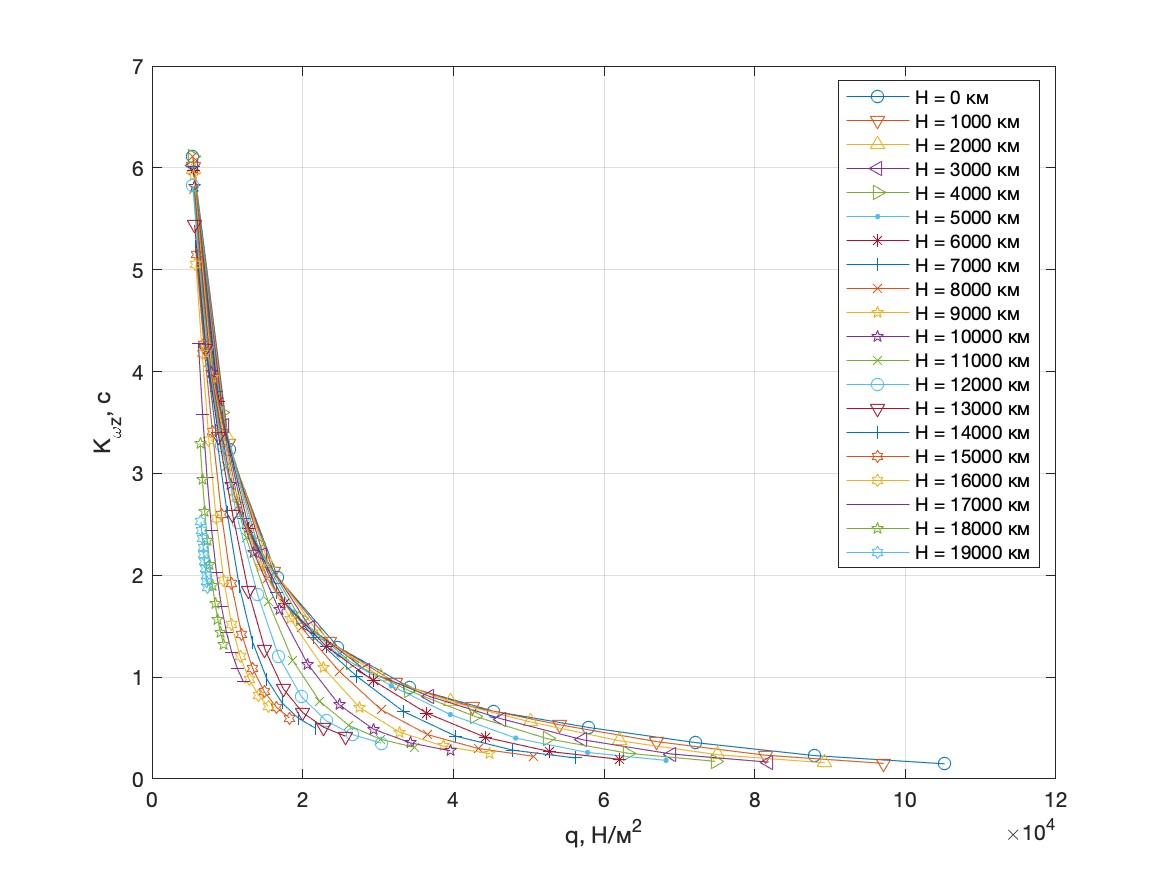
\includegraphics[width=6cm, height = 7cm]{../Оглавление/Part2/Sactions/Content/figures/K_wz.jpg}}
    \end{minipage}
    \begin{minipage}[c]{0.45\textwidth}
        \center{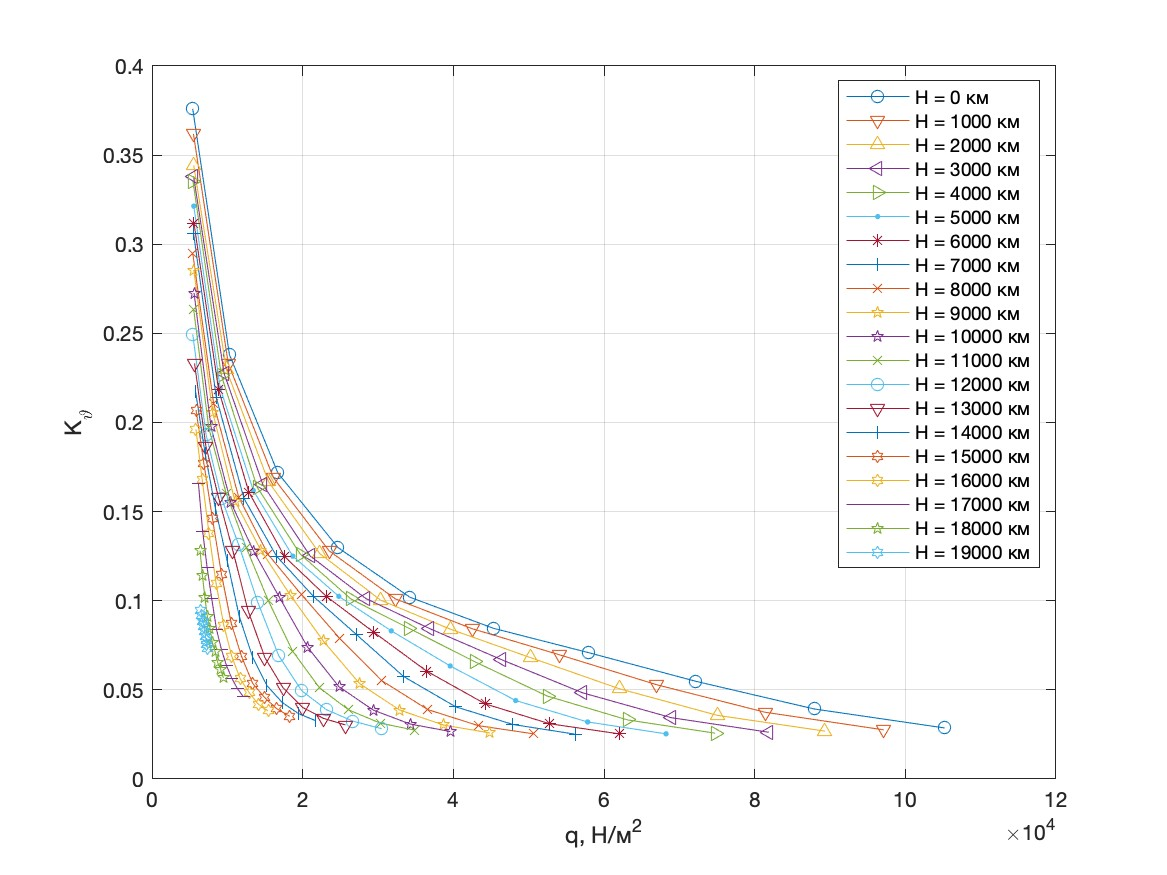
\includegraphics[width=6cm, height = 7cm]{../Оглавление/Part2/Sactions/Content/figures/K_v.jpg}}
    \end{minipage}
\end{frame}

\begin{frame}{Расчёт коэффициентов стабилизации системы}
    \begin{minipage}[c]{0.45\textwidth}
        \center{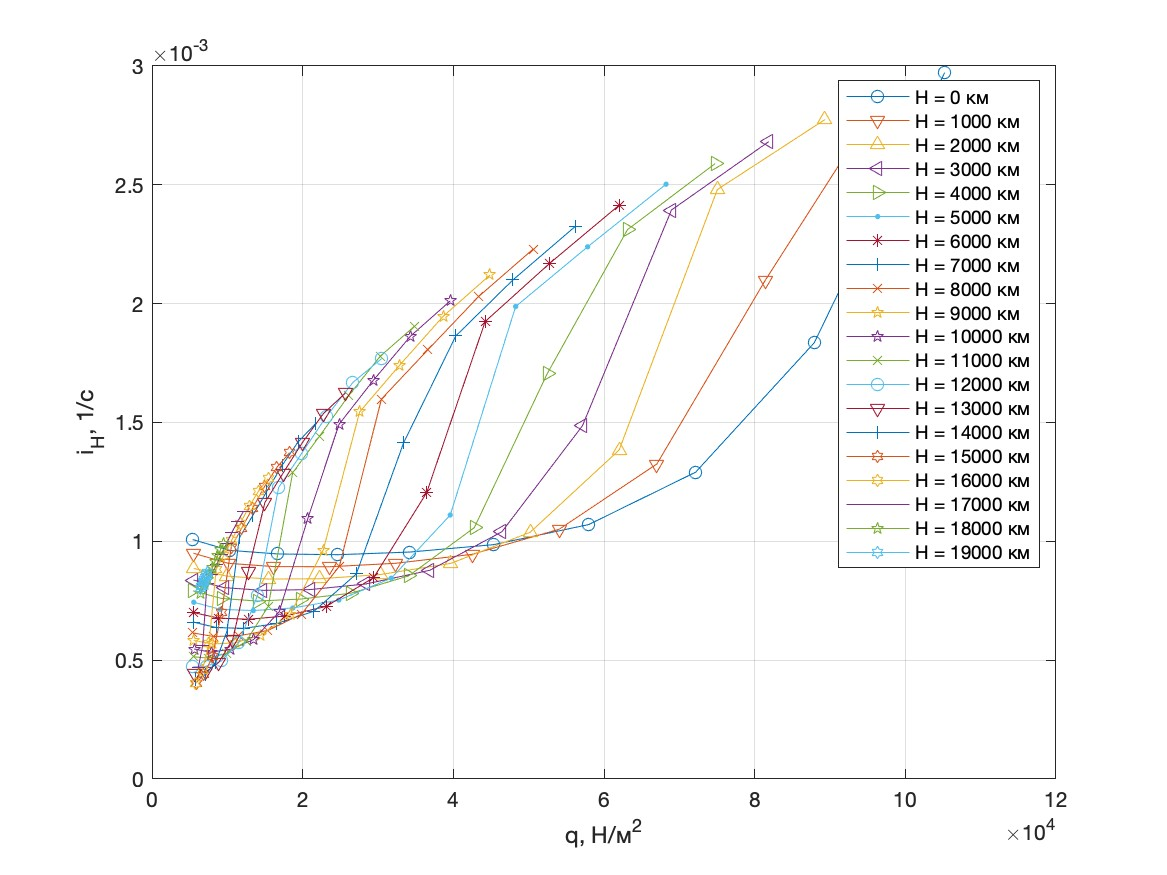
\includegraphics[width=6cm, height = 7cm]{../Оглавление/Part2/Sactions/Content/figures/i_H.jpg}}
    \end{minipage}
    \begin{minipage}[c]{0.45\textwidth}
        \center{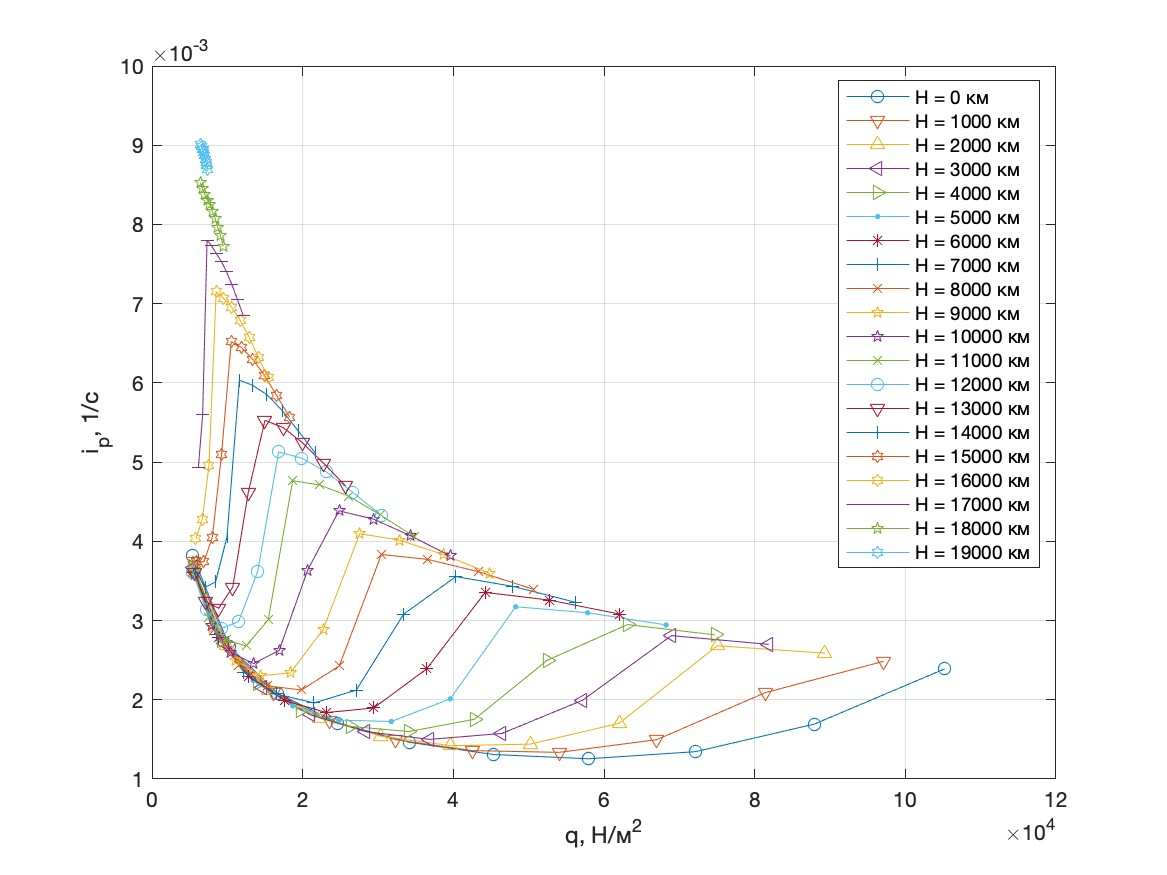
\includegraphics[width=6cm, height = 7cm]{../Оглавление/Part2/Sactions/Content/figures/i_p.jpg}}
    \end{minipage}
\end{frame}

\begin{frame}{Расчёт коэффициентов стабилизации системы}
    \begin{block}{Вывод}
        Полученные значения коэффициентов обратных связей были успешно найдены и применены на модели рассматриваемой 
        системы стабилизации вертикальной скорости в системе «Simulink». Моделирование показало, что коэффициенты найдены верно, 
        так как заданная вертикальная скорость равена вертикальной скорости на выходе из системы. 
        Более подробно будут показаны результаты моделирования и сама модель в разделе «Нелинейное моделирование».
    \end{block}
\end{frame}

\begin{frame}{Моделирование и анализ линейной и нелинейной САУ}
    \begin{itemize}
        \item <+-> []
        \item <+-> []
    \begin{block}{Основные положения}
        Целью частотного анализа является построение логарифмических амплитудных и фазовых частотных характеристик (ЛАФЧХ) 
        разомкнутых и замкнутых контуров управления до синтеза и после синтеза и проведение их сравнительного анализа.
    \end{block}
    \item <+-> []
    \begin{block}{Примечание}
        В данной призентации будет приведены частотные характеристики только для крейсерского полёта, 
        для остальных режимов всё аналогично.
    \end{block}
\end{itemize}
\end{frame}

\begin{frame}{Частотный аналез крейсерского режима полёта}
    \center{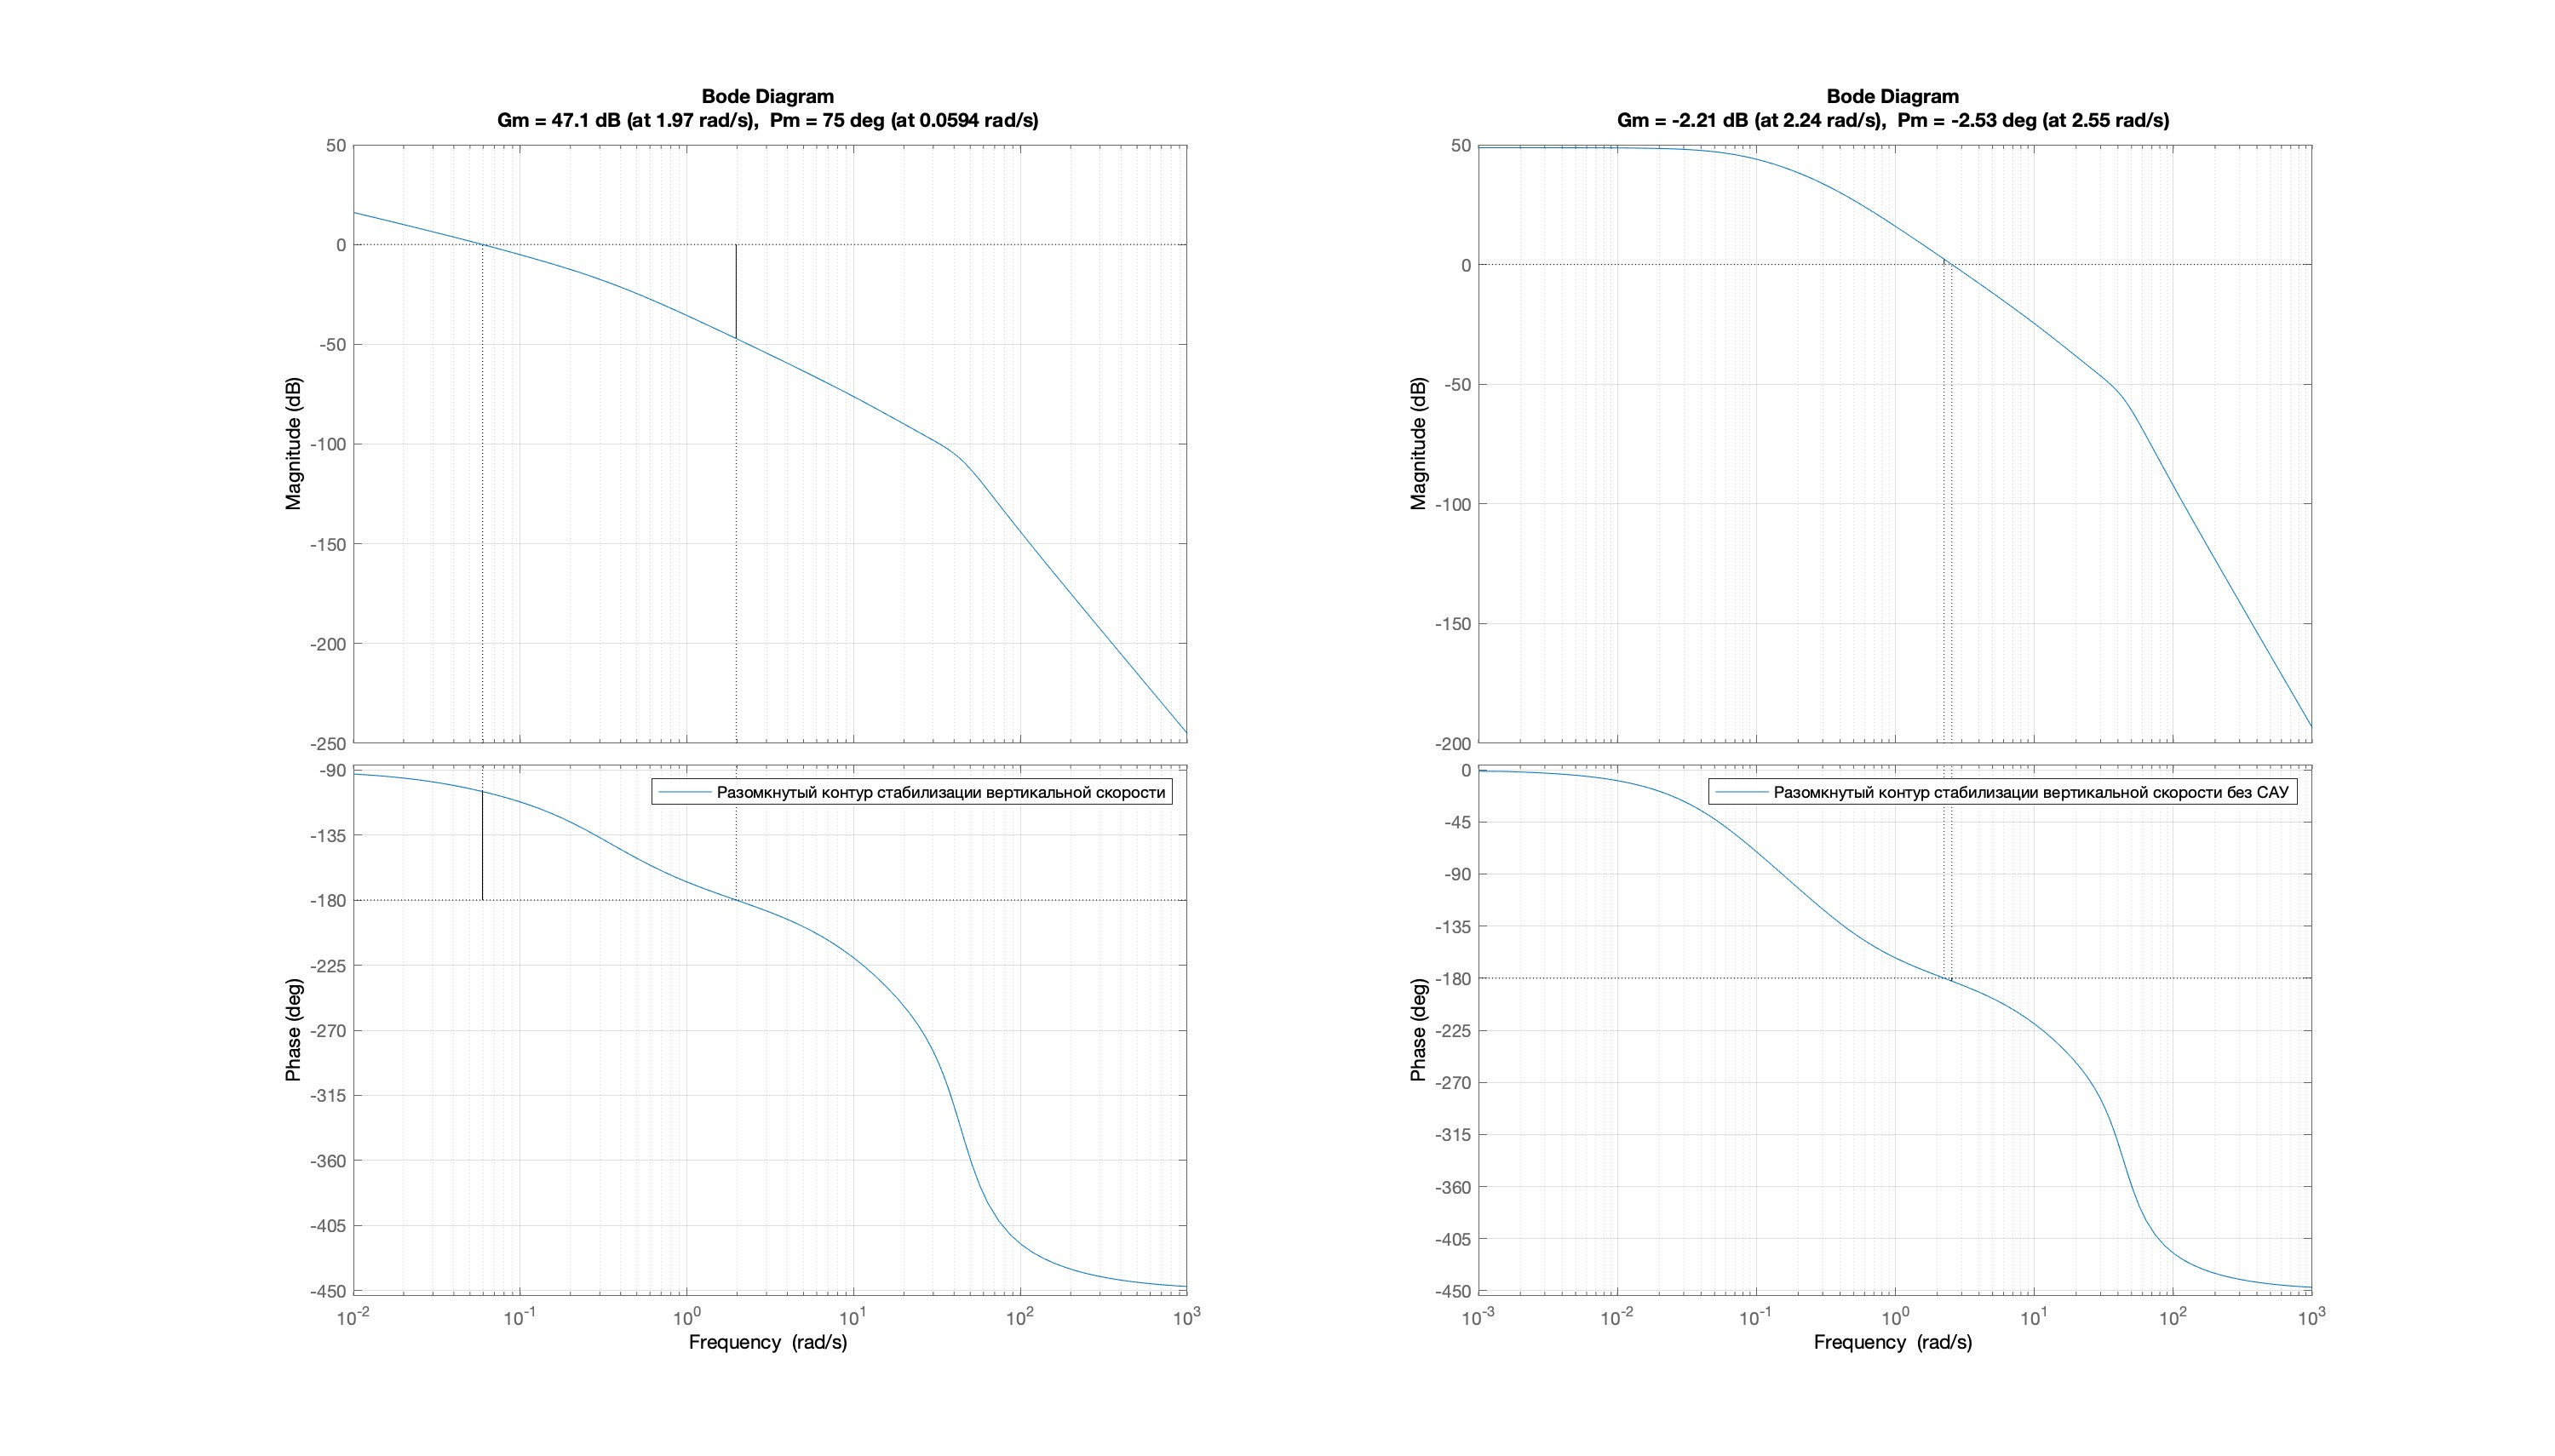
\includegraphics[width=10cm, height = 8cm]{../Оглавление/Part2/Sactions/Content/frequencies/Вертикальная скорость раз qKR.jpg}}
\end{frame}

\begin{frame}{Моделирование линейной и нелинейной САУ}
    \begin{block}{Общие положения}
        В данном разделе проводится анализ линейной и нелинейной САУ. В Simulink реализуется система управления на 
        крейсерском режиме полета. Крейсерскому режиму полета для самолета-прототипа Concorde соответствуют 
        М=0,982 и Н=17 км. 
    \end{block}
\end{frame}

